\documentclass[tikz,border=10pt]{standalone}
% Scale per STYLE METRICS: s=0.014981, centre (305,183.5) px
\usetikzlibrary{calc}
\begin{document}
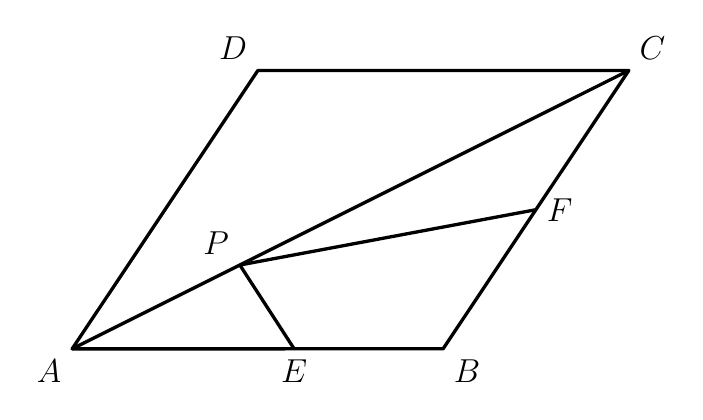
\begin{tikzpicture}[line width=1.2pt, line join=round, font=\fontsize{12}{14.4}\selectfont]
  % Vertices (converted from pixels)
  \coordinate (A) at (-3.553251544186164,-1.7603918093870905);
  \coordinate (B) at (1.1576039723386815,-1.7601259541386214);
  \coordinate (C) at (3.5164938967612556,1.7749776883834096);
  \coordinate (D) at (-1.1943616197635893,1.7747118331349405);
  % Points on segments
  \coordinate (E) at (-0.7339999868673199,-1.7602327060521143);
  \coordinate (P) at (-1.4235535000016022,-0.6958931555482805);
  \coordinate (F) at (2.3370687817187386,0.006954103607756668);

  % Parallelogram sides and diagonal
  \draw (A) -- (B) -- (C) -- (D) -- cycle;
  \draw (A) -- (C);
  % Auxiliary segments
  \draw (P) -- (E);
  \draw (P) -- (F);

  % Labels
  \node[below left] at (A) {$A$};
  \node[below right] at (B) {$B$};
  \node[above right] at (C) {$C$};
  \node[above left] at (D) {$D$};
  \node[below] at (E) {$E$};
  \node[right] at (F) {$F$};
  \node[above left] at (P) {$P$};
\end{tikzpicture}
\end{document}